
\section{Decay data} \label{data}
% 
% % \begin{longtable}{|c|c|c|c|c|} 
% % \caption{My caption}
% % \label{tab:dummy}
% % % \begin{tabular}{|c|c|c|c|c|}
% %    \hline
% %  
% % \end{longtable}
% Table of decay data  for observed gamma-rays. 
The   lifetimes and gamma-ray branching ratios  listed in these tables were used for all calculations of measured cross sections reported in this work, and have been taken from the most recent edition of  Nuclear Data Sheets for each  mass chain  \cite{Basunia2015,Firestone2007,Wang2017,Dong2015,Dong2014,JUNDE2008787,Junde2011,Bhat1998,Nesaraja2010,BAGLIN2002,Browne2013,Zuber20151,NICHOLS2012973,Singh2007,Browne2010,Tuli2003,McCutchan2015,Singh2014,NEGRET20151,Johnson2015,McCutchan2014,Singh2013,Browne1997,Baglin2013,Baglin2012,Baglin2011}. 


% \comment{I had to remove about 30 of the lines I used from this table (removing the weakest lines in nuclides with even more lines than shown here, but never removing lines in nuclides with only 2 or less), as even splitting the data into 2 tables created tables too large to fit on a single page.  My purpose here was 1) to show that I used multiple lines to quantify each nuclide (increasing confidence in results), and 2) to list all the used \ce{^{90}Mo} lines, since they form the basis of it as a monitor.  Is this good as is, or should it be pared down even more?}


% Preview source code for paragraph 0

\begin{table}[ht]
\centering
\caption{Decay data for gamma-rays observed in \ce{^{nat}Al}(p,x) and \ce{^{nat}Cu}(p,x).}
\label{tab:nudat_table_monitors}
\small
\begin{tabular}{@{}llll@{}}
\toprule
% \begin{tabular}{|c|c|c|c|}
% \hline 
Nuclide & Half-life & E$_\gamma$ (keV) & I$_\gamma$ (\%)\\
\midrule
\ce{^{22}Na} & 2.6018(22) y & 1274.537 & 99.940(14)\\
 
\ce{^{24}Na} & 14.997(12) h & 1368.626 & 99.9936(15)\\
 
\ce{^{51}Cr} & 27.704(3) d & 320.0824 & 9.910(10)\\
 
\ce{^{52m}Mn} & 21.1(2) m & 1434.0600 & 98.2(5)\\
 
\ce{^{52}Mn} & 5.591(3) d & 744.233 & 90.0(12)\\
 
 & 5.591(3) d & 935.544 & 94.5(13)\\
 
 & 5.591(3) d & 1246.278 & 4.21(7)\\
 
 & 5.591(3) d & 1434.092 & 100.0(14)\\
 
\ce{^{54}Mn} & 312.20(20) & 834.848 & 99.9760(10)\\
 
\ce{^{55}Co} & 17.53(3) h & 477.2 & 20.2(17)\\
 
 & 17.53(3) h & 931.1 & 75.0(35)\\
 
 & 17.53(3) h & 1316.6 & 7.1(3)\\
 
 & 17.53(3) h & 1408.5 & 16.9(8)\\
 
\ce{^{56}Ni} & 6.075(10) d & 158.38 & 98.8(10)\\
 
 & 6.075(10) d & 269.50 & 36.5(8)\\
 
 & 6.075(10) d & 480.44 & 36.5(8)\\
 
 & 6.075(10) d & 749.95 & 49.5(12)\\
 
 & 6.075(10) d & 811.85 & 86.0(9)\\
 
 & 6.075(10) d & 1561.80 & 14.0(6)\\
 
\ce{^{56}Co} & 77.236(26) d & 846.770 & 99.9399(2)\\
 
%  & 77.236(26) d & 977.372 & 1.421(6)\\
 
 & 77.236(26) d & 1037.843 & 14.05(4)\\
 
 & 77.236(26) d & 1238.288 & 66.46(12)\\
 
 & 77.236(26) d & 1360.212 & 4.283(12)\\
 
 & 77.236(26) d & 1771.357 & 15.41(6)\\
 
\ce{^{57}Ni} & 35.60(6) h & 127.164 & 16.7(5)\\
 
 & 35.60(6) h & 1377.63 & 81.7(24)\\
 
 & 35.60(6) h & 1757.55 & 5.75(20)\\
 
 & 35.60(6) h & 1919.52 & 12.3(4)\\
 
\ce{^{57}Co} & 271.74(6) d & 122.06065 & 85.60(17)\\
 
 & 271.74(6) d & 136.47356 & 10.68(8)\\
 
\ce{^{58}Co} & 70.86(6) d & 810.7593 & 99.450(10)\\
 
 & 70.86(6) d & 863.951 & 0.686(10)\\
 
%  & 70.86(6) d & 1674.725 & 0.517(10)\\
 
\ce{^{59}Fe} & 44.495(9) d & 1099.245 & 56.5(18)\\
 
 & 44.495(9) d & 1291.590 & 43.2(14)\\
 
\ce{^{60}Co} & 5.2714(5) y & 1173.228 & 99.85(3)\\
 
 & 5.2714(5) y & 1332.492 & 99.9826(6)\\
 
\ce{^{61}Cu} & 3.339(8) h & 282.956 & 12.2(2.2)\\
 
 & 3.339(8) h & 373.050 & 2.1(4)\\
 
%  & 3.339(8) h & 588.605 & 1.17(21)\\
 
 & 3.339(8) h & 656.008 & 10.8(20)\\
 
 & 3.339(8) h & 1185.234 & 3.7(7)\\
 
\ce{^{62}Zn} & 9.193(15) h & 243.36 & 2.52(23)\\
 
 & 9.193(15) h & 246.95 & 1.90(18)\\
 
 & 9.193(15) h & 260.43 & 1.35(13)\\
 
%  & 9.193(15) h & 304.88 & 0.29(3)\\
 
%  & 9.193(15) h & 349.60 & 0.45(4)\\
 
 & 9.193(15) h & 394.03 & 2.24(17)\\
 
 & 9.193(15) h & 548.35 & 15.3(14)\\
 
 & 9.193(15) h & 596.56 & 26.0(20)\\
 
%  & 9.193(15) h & 637.41 & 0.25(3)\\
 
\ce{^{64}Cu} & 12.701(2) h & 1345.77 & 0.475(11)\\
 
\ce{^{65}Zn} & 243.93(9) d & 1115.539 & 50.04(10)\\
\bottomrule
\end{tabular}
\end{table}



\begin{table}[ht]
\centering
\caption{Decay data for gamma-rays observed in \ce{^{nat}Nb}(p,x).}
\label{tab:nudat_table_nb}
\small
\begin{tabular}{@{}llll@{}}
\toprule
% \begin{tabular}{|c|c|c|c|}
% \hline 
Nuclide & Half-life & E$_\gamma$ (keV) & I$_\gamma$ (\%)\\
\midrule
\ce{^{82m}Rb} & 6.472(6) h & 554.35 & 62.4(9)\\
 
 & 6.472(6) h & 619.11 & 37.98(9)\\
 
%  & 6.472(6) h & 698.37 & 26.3(7)\\
 
 & 6.472(6) h & 776.52 & 84.39(21)\\
 
 & 6.472(6) h & 1044.08 & 32.07(8)\\
 
%  & 6.472(6) h & 1317.43 & 23.7(6)\\
 
\ce{^{83}Sr} & 32.41(3) h & 418.37 & 4.2(3)\\
 
 & 32.41(3) h & 762.65 & 26.7(22)\\
 
\ce{^{85m}Y} & 4.86(13) h & 231.7 & 22.8(22)\\
 
\ce{^{85}Y} & 2.68(5) h & 231.65 & 84(9)\\
 
 & 2.68(5) h & 913.89 & 9.0(9)\\
 
\ce{^{86}Zr} & 16.5(1) h & 242.8 & 95.84(2)\\
 
 & 16.5(1) h & 612.0 & 5.8(3)\\
 
% \ce{^{86}Y} & 14.74(2) h & 187.87 & 1.26(4)\\
\ce{^{86}Y}  & 14.74(2) h & 443.13 & 16.9(5)\\

 
%  & 14.74(2) h & 190.80 & 1.01(3)\\
 
%  & 14.74(2) h & 307.00 & 3.47(8)\\
 
%  & 14.74(2) h & 443.13 & 16.9(5)\\
 
%  & 14.74(2) h & 580.57 & 4.78(14)\\
 
%  & 14.74(2) h & 608.29 & 2.01(15)\\
 
 & 14.74(2) h & 627.72 & 32.6(1)\\
 
%  & 14.74(2) h & 703.33 & 15.4(4)\\
 
%  & 14.74(2) h & 709.90 & 2.62(8)\\
 
%  & 14.74(2) h & 767.63 & 2.4(3)\\
 
%  & 14.74(2) h & 835.67 & 4.4(6)\\
 
%  & 14.74(2) h & 1024.04 & 3.79(17)\\
 
 & 14.74(2) h & 1076.63 & 82.5(4)\\
 
 & 14.74(2) h & 1153.05 & 30.5(9)\\
 
%  & 14.74(2) h & 1163.03 & 1.18(4)\\
%  
%  & 14.74(2) h & 1253.11 & 1.53(5)\\
 
%  & 14.74(2) h & 1349.15 & 2.95(9)\\
 
 & 14.74(2) h & 1854.38 & 17.2(5)\\
 
 & 14.74(2) h & 1920.72 & 20.8(7)\\
 
\ce{^{87}Zr} & 1.68(1) h & 380.79 & 62.79(10)\\
 
 & 1.68(1) h & 1227.0 & 2.80(4)\\
 
\ce{^{87m}Y} & 13.37(1) h & 380.79 & 78.05(8)\\
 
\ce{^{87}Y} & 79.8(3) h & 388.5276 & 82.2(7)\\
 
 & 79.8(3) h & 484.805 & 89.8(9)\\
 
\ce{^{88}Zr} & 83.4(3) d & 392.87 & 97.29(14)\\
 
\ce{^{88}Y} & 106.627(21) d & 898.042 & 93.7(3)\\
 
 & 106.627(21) d & 1836.063 & 99.2(3)\\
 
\ce{^{89m}Nb} & 66(2) m & 588.0 & 95.57(13)\\
 
\ce{^{89}Nb} & 2.03(7) h & 1511.4 & 1.9(4)\\
 
 & 2.03(7) h & 1627.2 & 3.5(7)\\
 
 & 2.03(7) h & 1833.4 & 3.3(7)\\
 
\ce{^{89}Zr} & 78.41(12) h & 909.15 & 99.04(3)\\
 
 & 78.41(12) h & 1713.0 & 0.745(13)\\
 
%  & 78.41(12) h & 1744.5 & 0.123(4)\\
 
\ce{^{90}Mo} & 5.56(9) h & 122.370 & 64(3)\\
 
 & 5.56(9) h & 162.93 & 6.0(6)\\
 
 & 5.56(9) h & 203.13 & 6.4(6)\\
 
 & 5.56(9) h & 257.34 & 78(4)\\
 
 & 5.56(9) h & 323.20 & 6.3(6)\\
 
 & 5.56(9) h & 472.2 & 1.42(16)\\
 
 & 5.56(9) h & 941.5 & 5.5(7)\\
 
\ce{^{90}Nb} & 14.6(5) h & 132.716 & 4.13(4)\\
 
 & 14.6(5) h & 141.178 & 66.8(7)\\
 
%  & 14.6(5) h & 890.64 & 1.80(4)\\
 
 & 14.6(5) h & 1611.76 & 2.38(7)\\
 
%  & 14.6(5) h & 1913.194 & 1.280(17)\\
 
\ce{^{91m}Nb} & 60.86(22) d & 104.62 & 0.574(1)\\
 
 & 60.86(22) d & 1204.67 & 2.0(3)\\
 
\ce{^{92m}Nb} & 10.15(2) d & 912.6 & 1.78(10)\\
 
 & 10.15(2) d & 934.44 & 99.15(4)\\
 
\ce{^{93m}Mo} & 6.85(7) d & 263.049 & 57.4(11)\\
 
 & 6.85(7) d & 684.693 & 99.9(8)\\
 
 & 6.85(7) d & 1477.138 & 99.1(11)\\
\bottomrule
\end{tabular}
\end{table}


% 
% 
\section{Measured excitation functions} \label{fit_figures}

Figures of the cross sections measured in this work are presented here, in comparison with literature data \cite{Albouy1963,PhysRev.162.1055,PhysRevC.6.1235,Grutter1982,Greenwood1984,Aleksandrov1987,levkovski1991cross,Mills1992,MICHEL1997153,Fassbender1997,Ido2002,sisterson2002selected,YashimaH2003,A2006,Ditroi2008,Ditroi2009,steyn2011excitation,Titarenko2011,Shahid2015,Garrido2016,Graves2016}, the TENDL-2015 data library \cite{Koning2012}, and the reaction modeling codes CoH-3.5.1, EMPIRE-3.2.3, and TALYS-1.8 \cite{KAWANO2010,Herman2007,Koning2012}.

% \comment{Add in CoH model output from Toshihiko to all plots}




% \comment{Fix a few figure labels (c/i) based on Jon;s email}

% Prevent ''overfull hbox'' warnings for < 5pt overflow 
% \hfuzz=10pt 

\begin{figure*}
    \sloppy
    \centering
    \subfloat{
        \centering
%         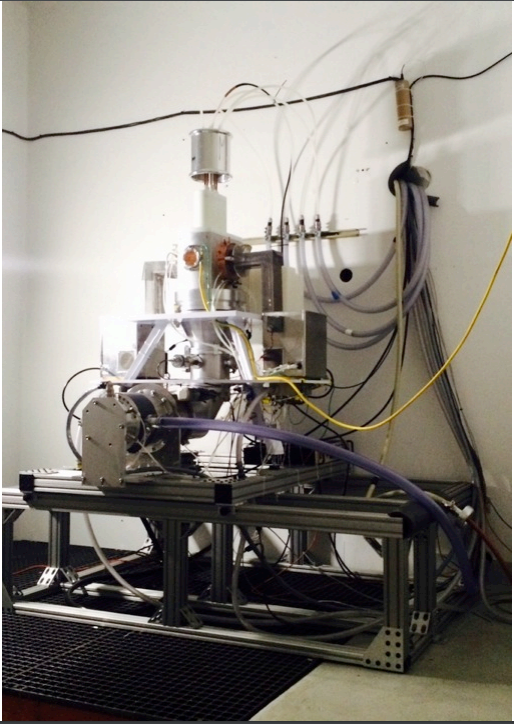
\includegraphics[width=\columnwidth]{./figures/Capture.PNG}
        \subfigimg[width=0.5\textwidth]{}{./figures/51Cr.pdf}{50}
%         \caption{ Decay curve for the isomeric transition of \ce{^{115m}In}.}
%         \refstepcounter{subfigure}
%          \label{fig:51Cr}%
%         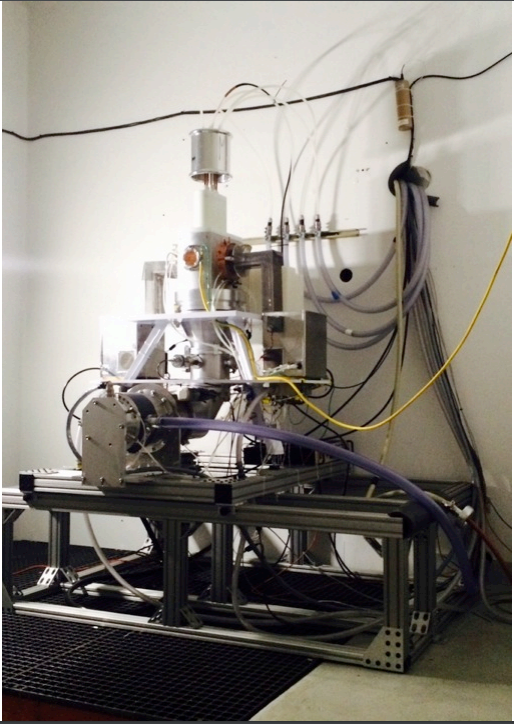
\includegraphics[width=\columnwidth]{./figures/Capture.PNG}
%         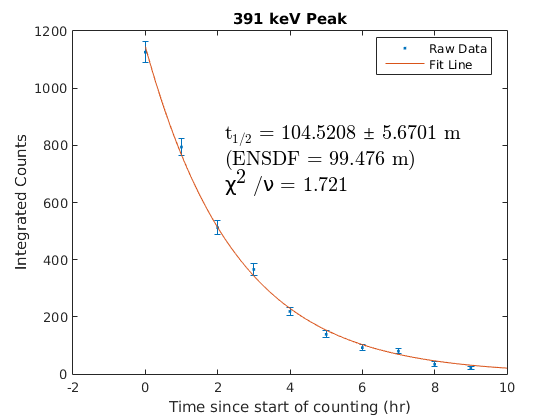
\includegraphics[scale=0.6]{./figures/391keV_curve2.png}
        \subfigimg[width=0.5\textwidth]{}{./figures/52Mn.pdf}{50}
%         \caption{ Decay curve for the isomeric transition of \ce{^{113m}In}.}
%         \refstepcounter{subfigure}
%          \label{fig:52Mn}
   \hspace{-10pt}}%
    \\
    \subfloat{
        \centering
%         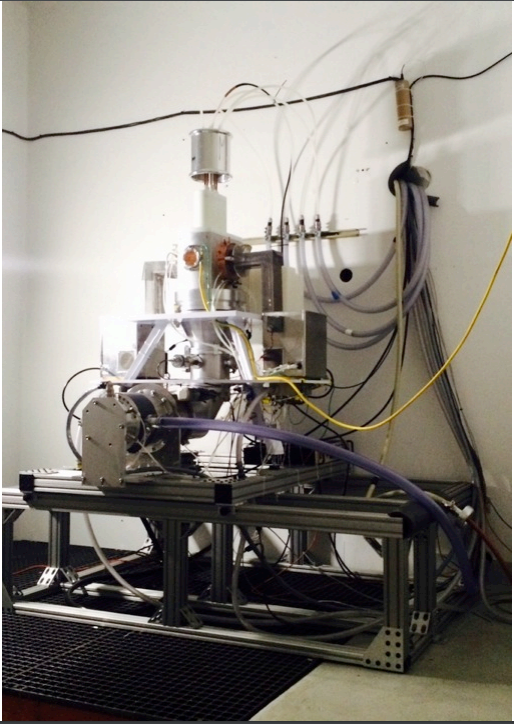
\includegraphics[width=\columnwidth]{./figures/Capture.PNG}
        \subfigimg[width=0.5\textwidth]{}{./figures/52gMn.pdf}{50}
%         \caption{ Decay curve for the isomeric transition of \ce{^{115m}In}.}
%         \refstepcounter{subfigure}
%          \label{fig:52gMn}%
%         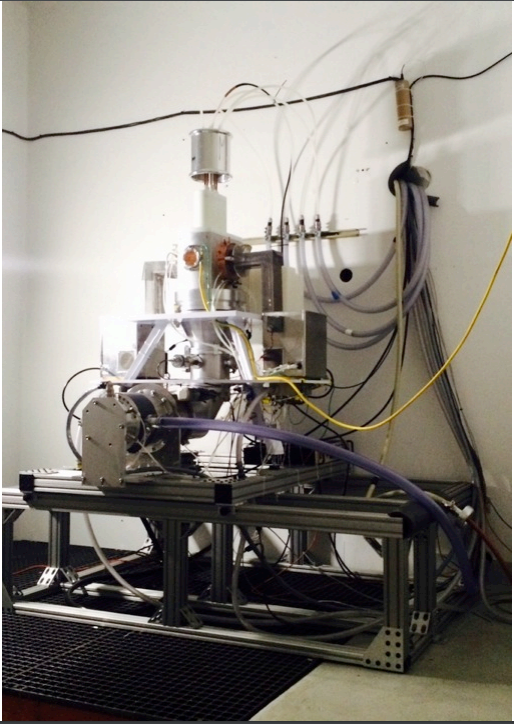
\includegraphics[width=\columnwidth]{./figures/Capture.PNG}
%         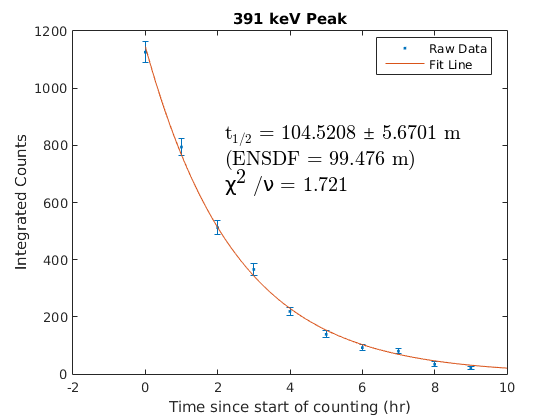
\includegraphics[scale=0.6]{./figures/391keV_curve2.png}
        \subfigimg[width=0.5\textwidth]{}{./figures/52mMn.pdf}{50}
%         \caption{ Decay curve for the isomeric transition of \ce{^{113m}In}.}
%         \refstepcounter{subfigure}
%          \label{fig:52mMn}
   \hspace{-10pt}}%
    \\
    \subfloat{
        \centering
%         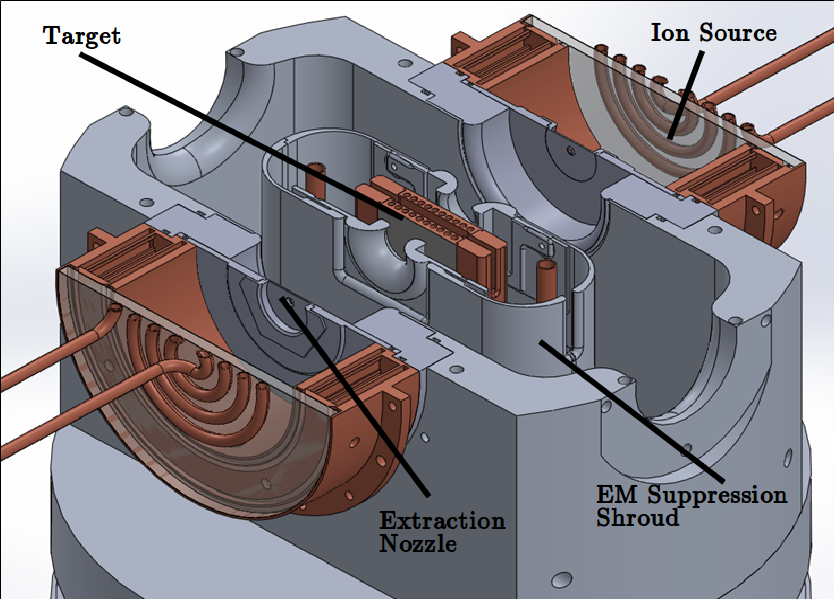
\includegraphics[width=\textwidth]{./figures/target2.png}
        \subfigimg[width=0.5\textwidth]{}{./figures/54Mn.pdf}{50}
%         \caption{Decay curve for the $\beta^-$ decay of \ce{^{116}In}.}
        %         \refstepcounter{subfigure}
%          \label{fig:54Mn}
%
%         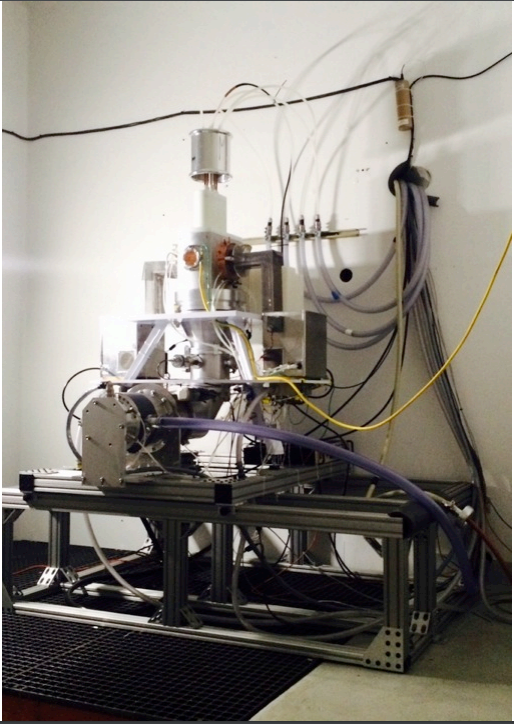
\includegraphics[width=\columnwidth]{./figures/Capture.PNG}
        \subfigimg[width=0.5\textwidth]{}{./figures/55Co.pdf}{50}
%         \caption{ Decay curve for the $\beta^+$ decay of \ce{^{64}Cu}.}
%         \refstepcounter{subfigure} 
%         \label{fig:55Co}
   \hspace{-10pt}}%
%     \caption{Decay curves used to verify photopeak transition assignment. (a) Decay curve for the isomeric transition of \ce{^{115m}In}, (b) decay curve for the isomeric transition of \ce{^{113m}In}, (c) decay curve for the $\beta^-$ decay of \ce{^{116}In}, and (d) decay curve for the $\beta^+$ decay of \ce{^{64}Cu}.}
     \phantomcaption{}\label{fig:xs_curves_p1}
\end{figure*}




\begin{figure*}
    \centering
    \subfloat{
        \centering
%         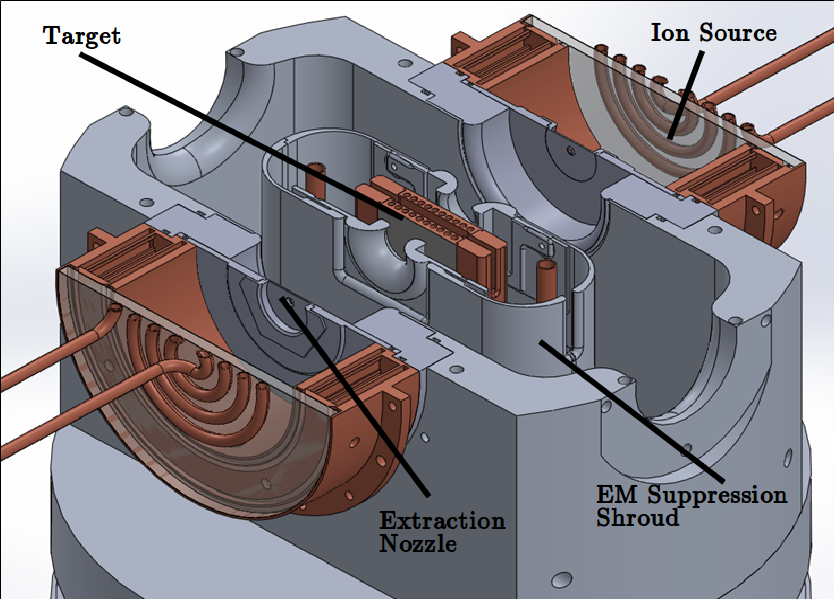
\includegraphics[width=\textwidth]{./figures/target2.png}
        \subfigimg[width=0.5\textwidth]{}{./figures/56Ni.pdf}{50}
%         \caption{Decay curve for the $\beta^-$ decay of \ce{^{116}In}.}
        %         \refstepcounter{subfigure}
%          \label{fig:56Ni}
%
%         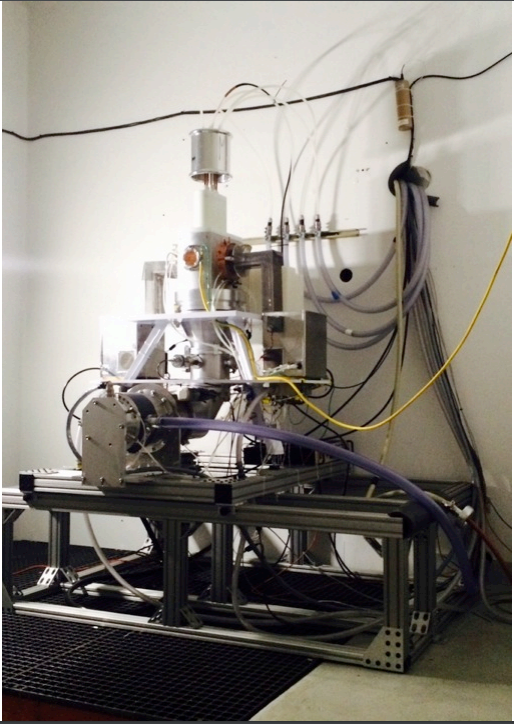
\includegraphics[width=\columnwidth]{./figures/Capture.PNG}
        \subfigimg[width=0.5\textwidth]{}{./figures/57Co.pdf}{50}
%         \caption{ Decay curve for the $\beta^+$ decay of \ce{^{64}Cu}.}
%         \refstepcounter{subfigure}
%         \label{fig:57Co}
   \hspace{-10pt}}%
    \\
    \subfloat{
        \centering
%         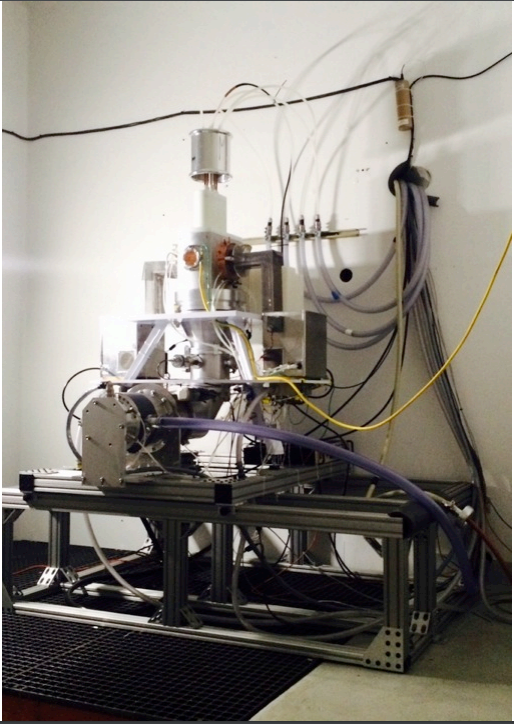
\includegraphics[width=\columnwidth]{./figures/Capture.PNG}
        \subfigimg[width=0.5\textwidth]{}{./figures/57Ni.pdf}{50}
%         \caption{ Decay curve for the isomeric transition of \ce{^{115m}In}.}
%         \refstepcounter{subfigure}
%          \label{fig:57Ni}%
%         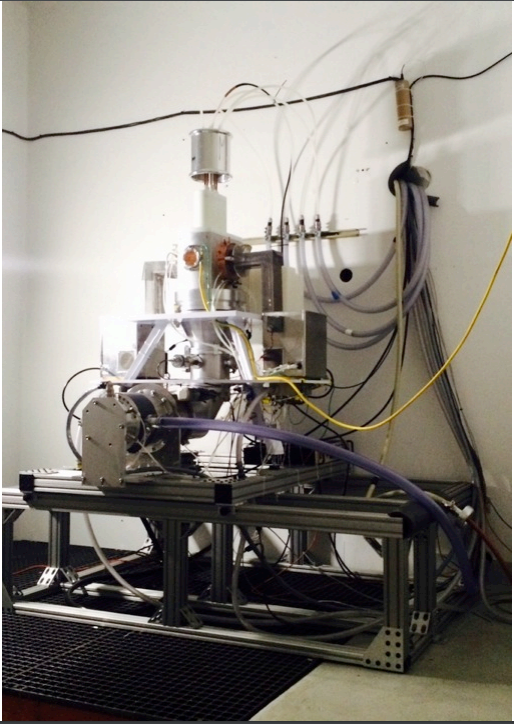
\includegraphics[width=\columnwidth]{./figures/Capture.PNG}
%         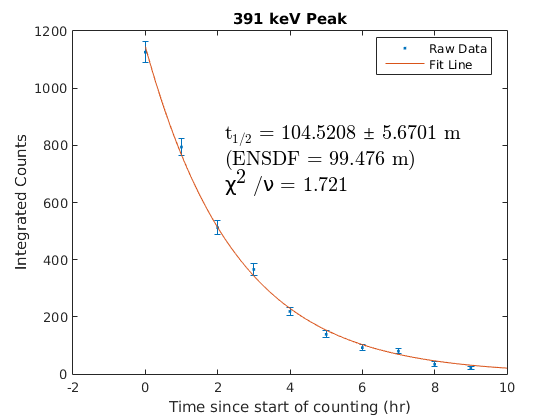
\includegraphics[scale=0.6]{./figures/391keV_curve2.png}
        \subfigimg[width=0.5\textwidth]{}{./figures/58Co.pdf}{50}
%         \caption{ Decay curve for the isomeric transition of \ce{^{113m}In}.}
%         \refstepcounter{subfigure}
%          \label{fig:58Co}
   \hspace{-10pt}}%
    \\
    \subfloat{
        \centering
%         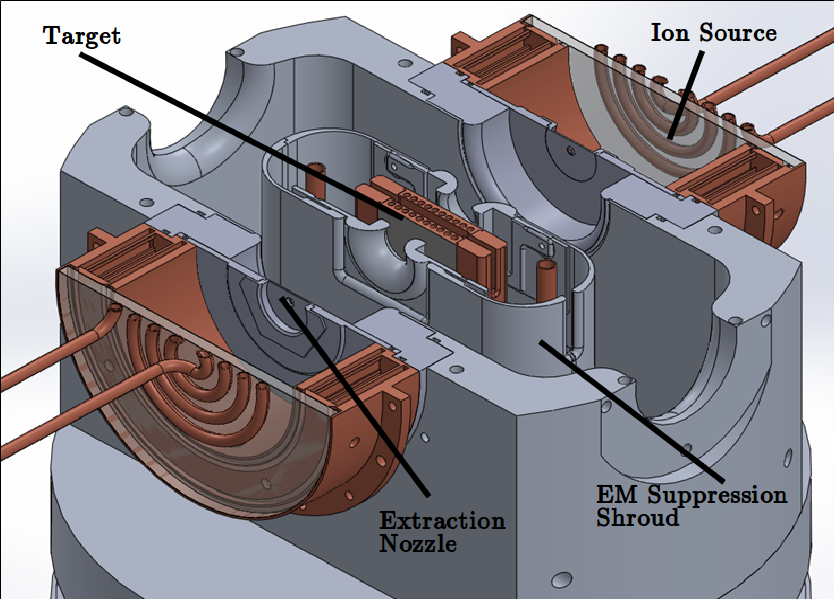
\includegraphics[width=\textwidth]{./figures/target2.png}
        \subfigimg[width=0.5\textwidth]{}{./figures/58gCo.pdf}{50}
%         \caption{Decay curve for the $\beta^-$ decay of \ce{^{116}In}.}
        %         \refstepcounter{subfigure}
%          \label{fig:58gCo}
%
%         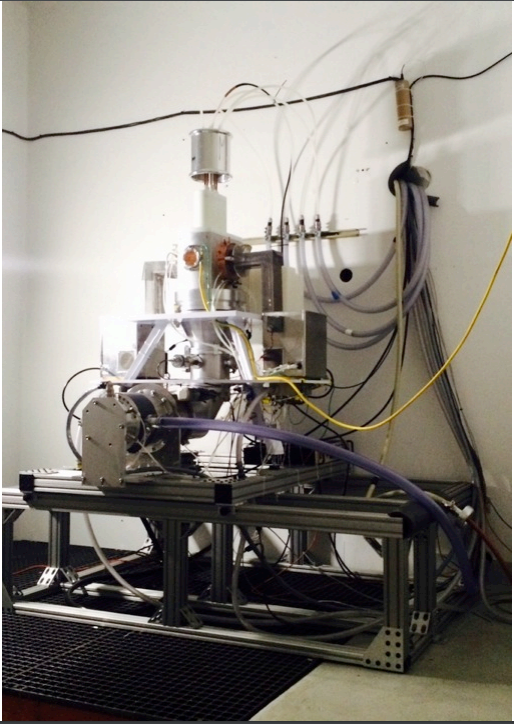
\includegraphics[width=\columnwidth]{./figures/Capture.PNG}
        \subfigimg[width=0.5\textwidth]{}{./figures/58mCo.pdf}{50}
%         \caption{ Decay curve for the $\beta^+$ decay of \ce{^{64}Cu}.}
%         \refstepcounter{subfigure}
%         \label{fig:58mCo}
   \hspace{-10pt}}%
%     \caption{Decay curves used to verify photopeak transition assignment. (a) Decay curve for the isomeric transition of \ce{^{115m}In}, (b) decay curve for the isomeric transition of \ce{^{113m}In}, (c) decay curve for the $\beta^-$ decay of \ce{^{116}In}, and (d) decay curve for the $\beta^+$ decay of \ce{^{64}Cu}.}
     \phantomcaption{}\label{fig:xs_curves_p2}
\end{figure*}



\begin{figure*}
    \centering
    \subfloat{
        \centering
%         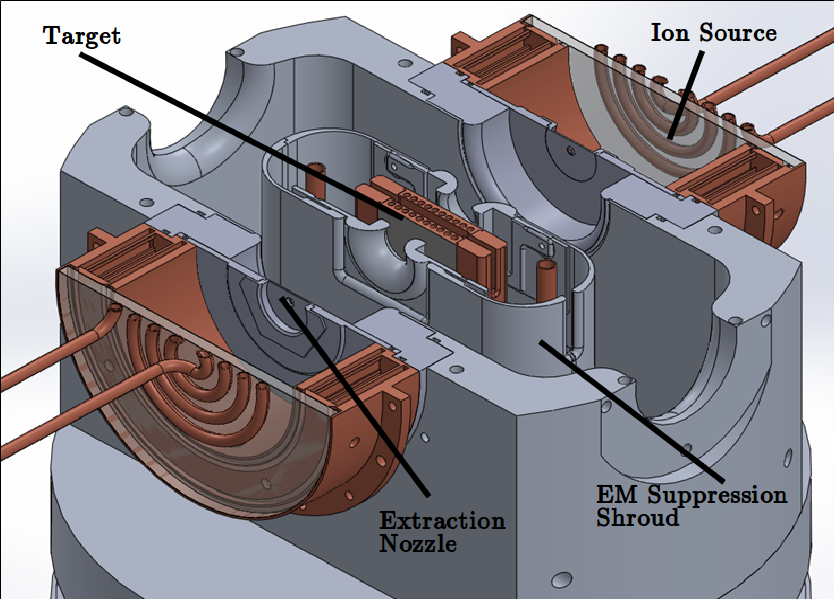
\includegraphics[width=\textwidth]{./figures/target2.png}
        \subfigimg[width=0.5\textwidth]{}{./figures/59Fe.pdf}{50}
%         \caption{Decay curve for the $\beta^-$ decay of \ce{^{116}In}.}
        %         \refstepcounter{subfigure}
%          \label{fig:59Fe}
%
%         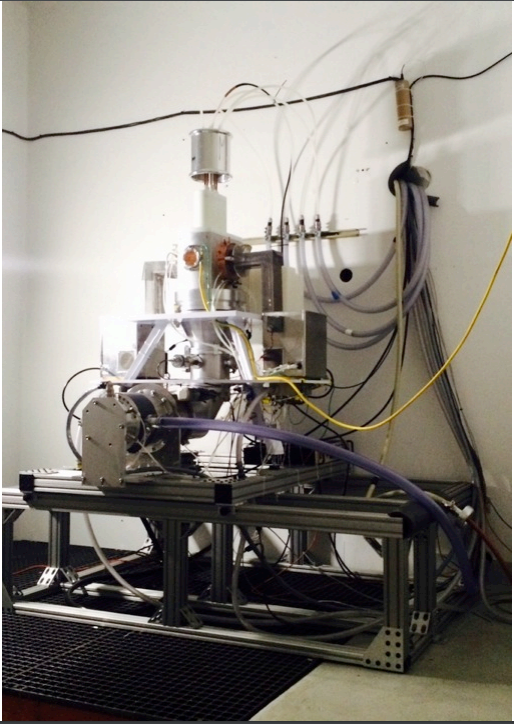
\includegraphics[width=\columnwidth]{./figures/Capture.PNG}
        \subfigimg[width=0.5\textwidth]{}{./figures/60Co.pdf}{50}
%         \caption{ Decay curve for the $\beta^+$ decay of \ce{^{64}Cu}.}
%         \refstepcounter{subfigure} 
%         \label{fig:60Co}
   \hspace{-10pt}}%
    \\
    \subfloat{
        \centering
%         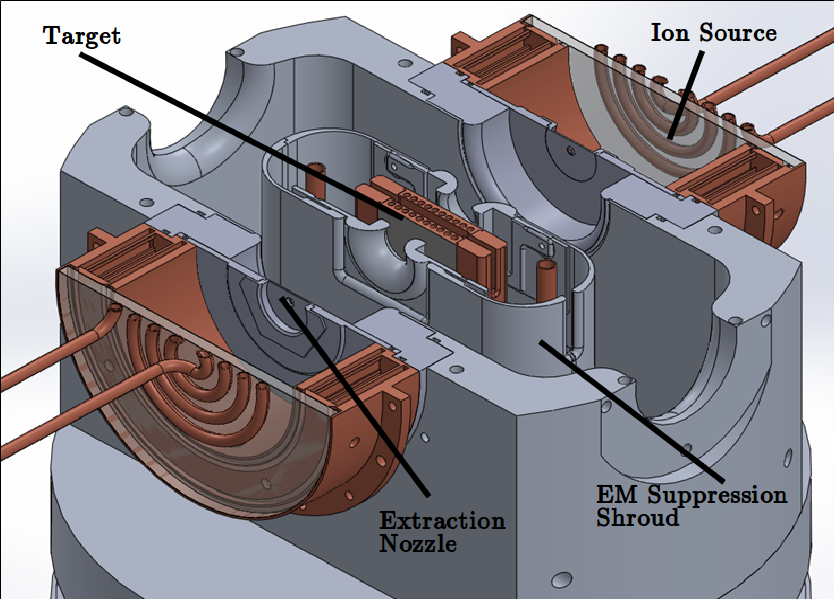
\includegraphics[width=\textwidth]{./figures/target2.png}
        \subfigimg[width=0.5\textwidth]{}{./figures/61Cu.pdf}{50}
%         \caption{Decay curve for the $\beta^-$ decay of \ce{^{116}In}.}
        %         \refstepcounter{subfigure}
%          \label{fig:61Cu}
%
%         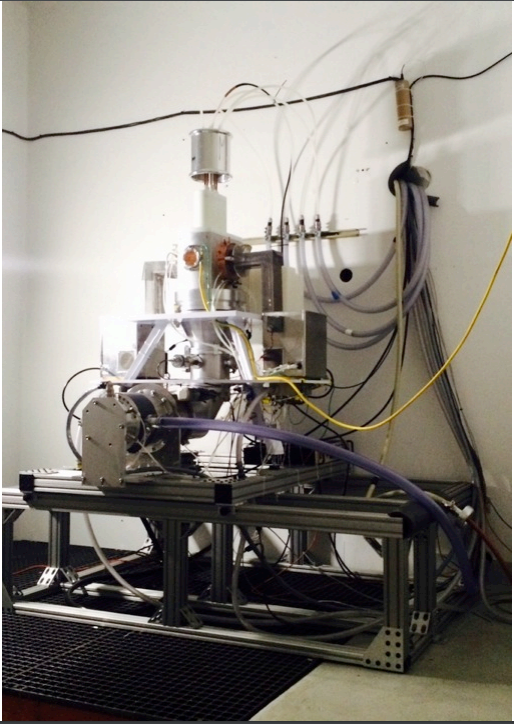
\includegraphics[width=\columnwidth]{./figures/Capture.PNG}
        \subfigimg[width=0.5\textwidth]{}{./figures/64Cu.pdf}{50}
%         \caption{ Decay curve for the $\beta^+$ decay of \ce{^{64}Cu}.}
%         \refstepcounter{subfigure}
%         \label{fig:64Cu}
   \hspace{-10pt}}%
    \\
    \subfloat{
        \centering
%         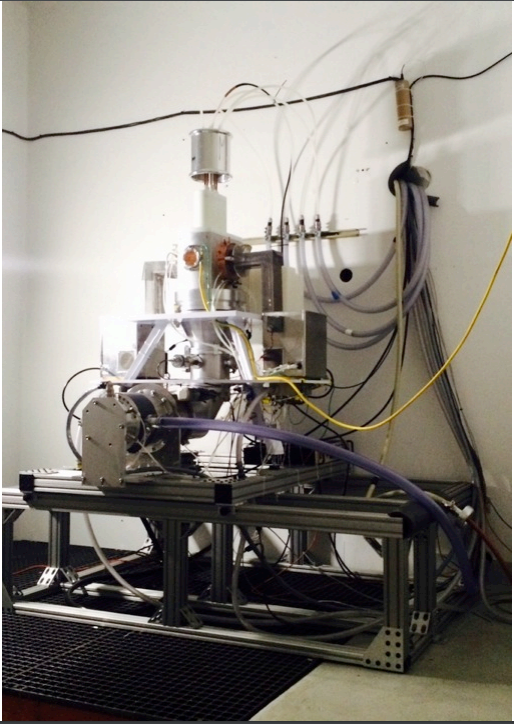
\includegraphics[width=\columnwidth]{./figures/Capture.PNG}
        \subfigimg[width=0.5\textwidth]{}{./figures/82mRb.pdf}{50}
%         \caption{ Decay curve for the isomeric transition of \ce{^{115m}In}.}
%         \refstepcounter{subfigure}
%          \label{fig:82mRb}%
%         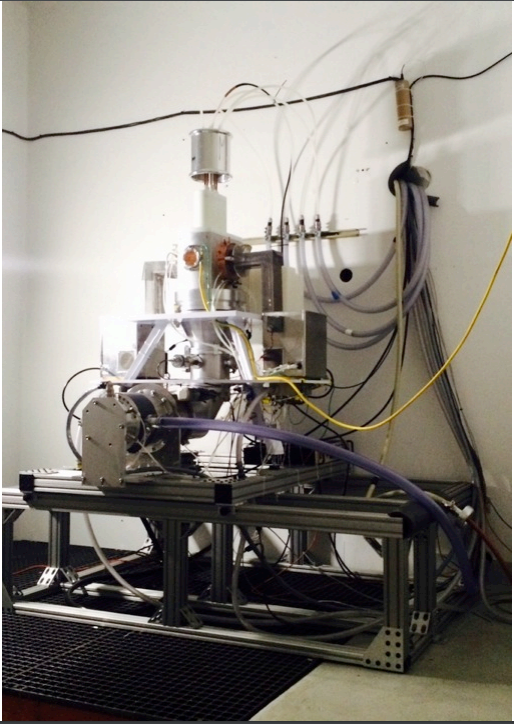
\includegraphics[width=\columnwidth]{./figures/Capture.PNG}
%         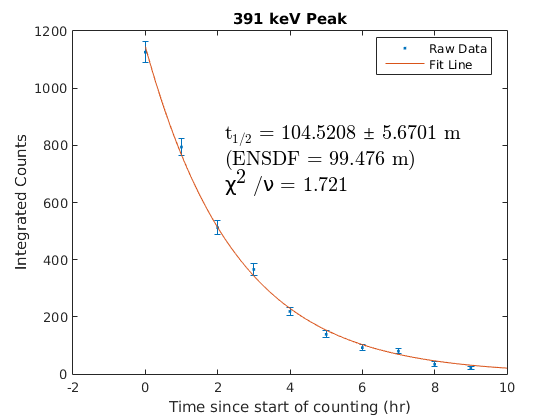
\includegraphics[scale=0.6]{./figures/391keV_curve2.png}
        \subfigimg[width=0.5\textwidth]{}{./figures/83Sr.pdf}{50}
%         \caption{ Decay curve for the isomeric transition of \ce{^{113m}In}.}
%         \refstepcounter{subfigure}
%          \label{fig:83Sr}
   \hspace{-10pt}}%
%     \caption{Decay curves used to verify photopeak transition assignment. (a) Decay curve for the isomeric transition of \ce{^{115m}In}, (b) decay curve for the isomeric transition of \ce{^{113m}In}, (c) decay curve for the $\beta^-$ decay of \ce{^{116}In}, and (d) decay curve for the $\beta^+$ decay of \ce{^{64}Cu}.}
     \phantomcaption{}\label{fig:xs_curves_p3}
\end{figure*}



\begin{figure*}
    \centering
    \subfloat{
        \centering
%         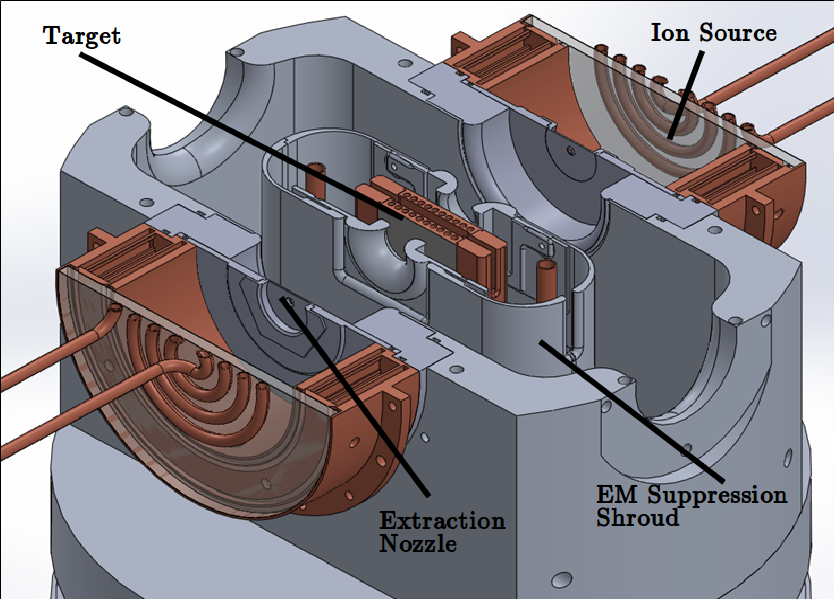
\includegraphics[width=\textwidth]{./figures/target2.png}
        \subfigimg[width=0.5\textwidth]{}{./figures/85Y.pdf}{50}
%         \caption{Decay curve for the $\beta^-$ decay of \ce{^{116}In}.}
        %         \refstepcounter{subfigure}
%          \label{fig:85Y}
%
%         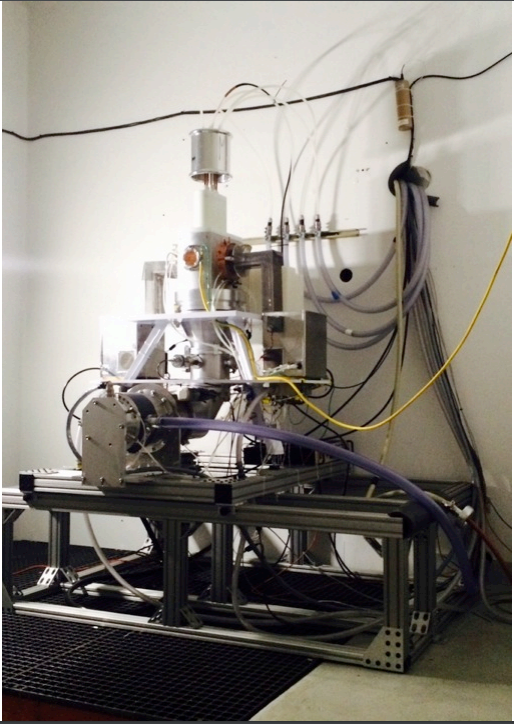
\includegraphics[width=\columnwidth]{./figures/Capture.PNG}
        \subfigimg[width=0.5\textwidth]{}{./figures/85gY.pdf}{50}
%         \caption{ Decay curve for the $\beta^+$ decay of \ce{^{64}Cu}.}
%         \refstepcounter{subfigure} 
%         \label{fig:85gY}
   \hspace{-10pt}}%
    \\
    \subfloat{
        \centering
%         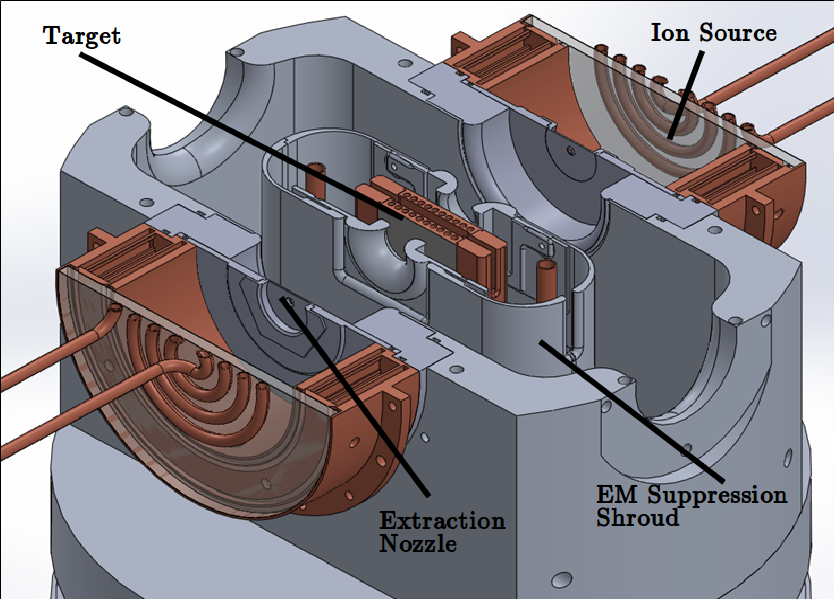
\includegraphics[width=\textwidth]{./figures/target2.png}
        \subfigimg[width=0.5\textwidth]{}{./figures/85mY.pdf}{50}
%         \caption{Decay curve for the $\beta^-$ decay of \ce{^{116}In}.}
        %         \refstepcounter{subfigure}
%          \label{fig:85mY}
%    }
%      \subfloat{
%         \centering
% %         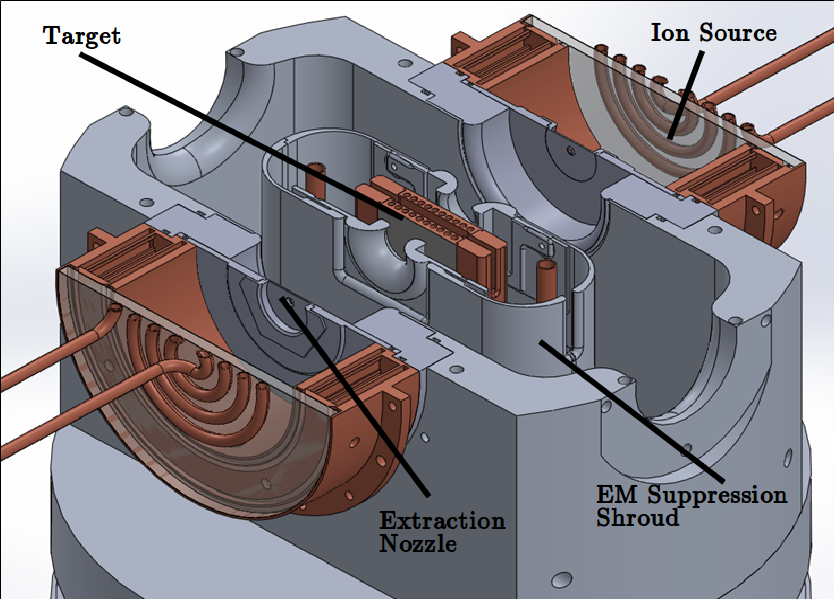
\includegraphics[width=\textwidth]{./figures/target2.png}
%         \subfigimg[width=0.5\textwidth]{}{./figures/86Y.pdf}{50}
% %         \caption{Decay curve for the $\beta^-$ decay of \ce{^{116}In}.}
%         %         \refstepcounter{subfigure}
%          \label{fig:86Y}
%    }
%     \\
%     \subfloat{
%         \centering
%         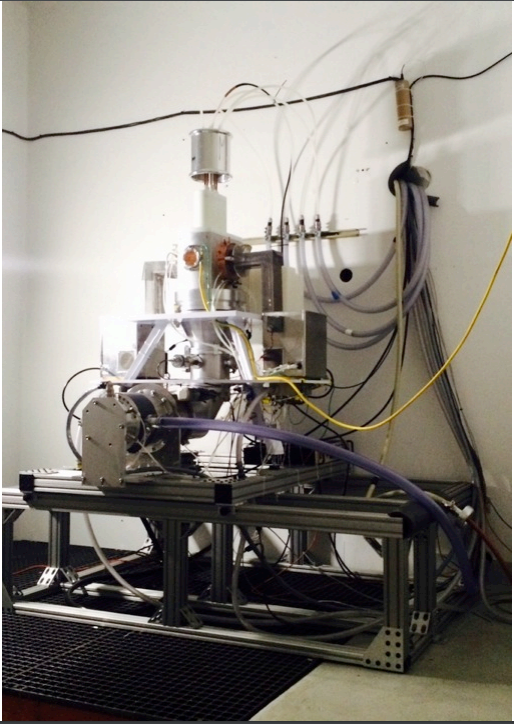
\includegraphics[width=\columnwidth]{./figures/Capture.PNG}
        \subfigimg[width=0.5\textwidth]{}{./figures/86Zr.pdf}{50}
%         \caption{ Decay curve for the $\beta^+$ decay of \ce{^{64}Cu}.}
%         \refstepcounter{subfigure}
%         \label{fig:86Zr}
   \hspace{-10pt}}%
    \\
    \subfloat{
        \centering
%         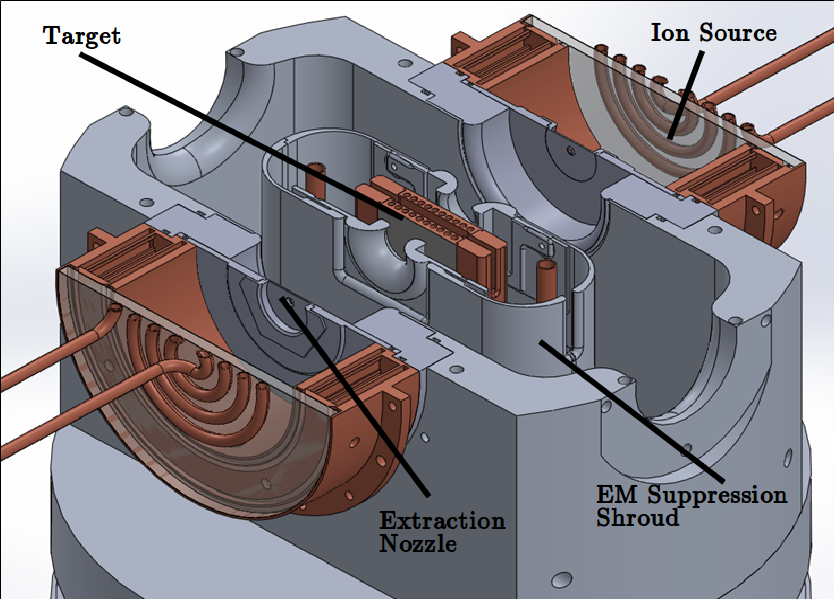
\includegraphics[width=\textwidth]{./figures/target2.png}
        \subfigimg[width=0.5\textwidth]{}{./figures/87Y.pdf}{50}
%         \caption{Decay curve for the $\beta^-$ decay of \ce{^{116}In}.}
        %         \refstepcounter{subfigure}
%          \label{fig:87Y}
%    }
%     \subfloat{
%         \centering
%         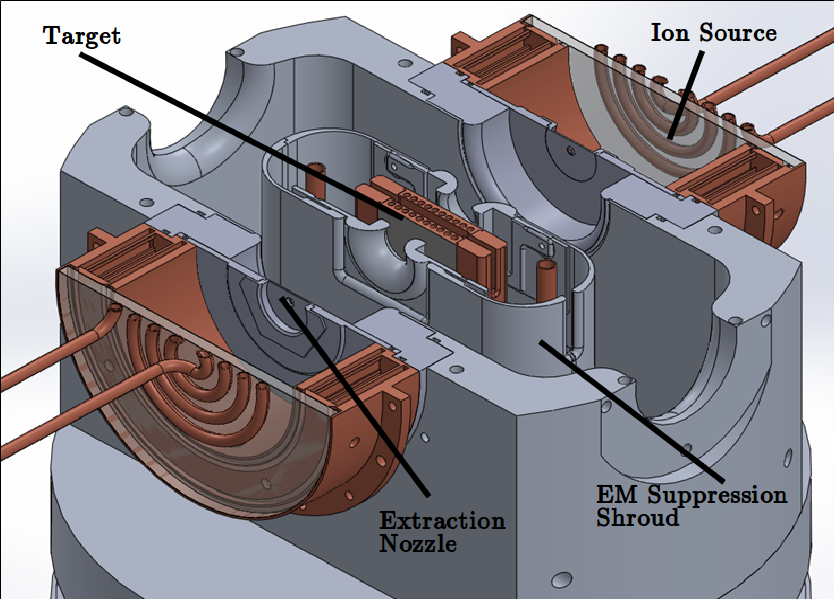
\includegraphics[width=\textwidth]{./figures/target2.png}
        \subfigimg[width=0.5\textwidth]{}{./figures/87gY.pdf}{50}
%         \caption{Decay curve for the $\beta^-$ decay of \ce{^{116}In}.}
        %         \refstepcounter{subfigure}
%          \label{fig:87gY}
   \hspace{-10pt}}
%     \caption{Decay curves used to verify photopeak transition assignment. (a) Decay curve for the isomeric transition of \ce{^{115m}In}, (b) decay curve for the isomeric transition of \ce{^{113m}In}, (c) decay curve for the $\beta^-$ decay of \ce{^{116}In}, and (d) decay curve for the $\beta^+$ decay of \ce{^{64}Cu}.}
     \phantomcaption{}\label{fig:xs_curves_p4}
\end{figure*}

\begin{figure*}
    \centering
     \subfloat{
        \centering
% %         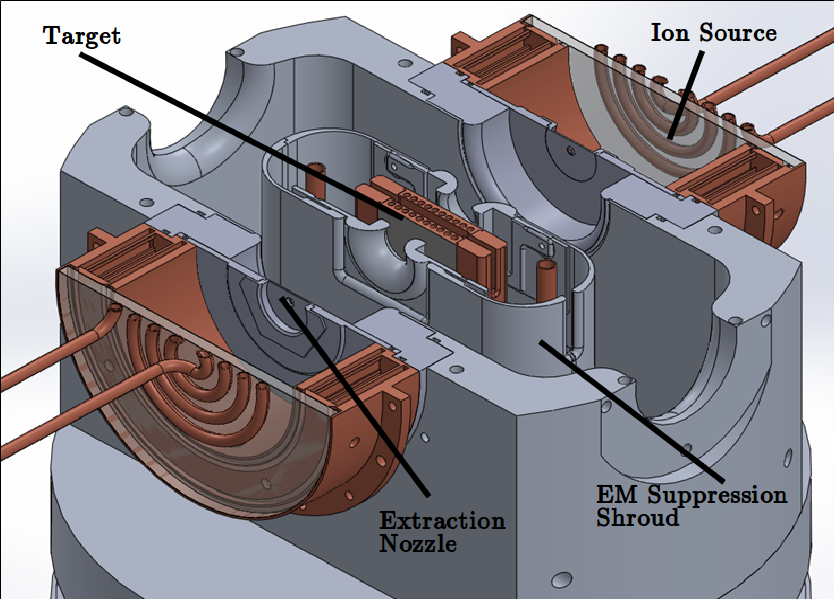
\includegraphics[width=\textwidth]{./figures/target2.png}
%         \subfigimg[width=0.5\textwidth]{}{./figures/87gY.pdf}{50}
% %         \caption{Decay curve for the $\beta^-$ decay of \ce{^{116}In}.}
%         %         \refstepcounter{subfigure}
%          \label{fig:87gY}
% %    }
%     \subfloat{
%         \centering
%         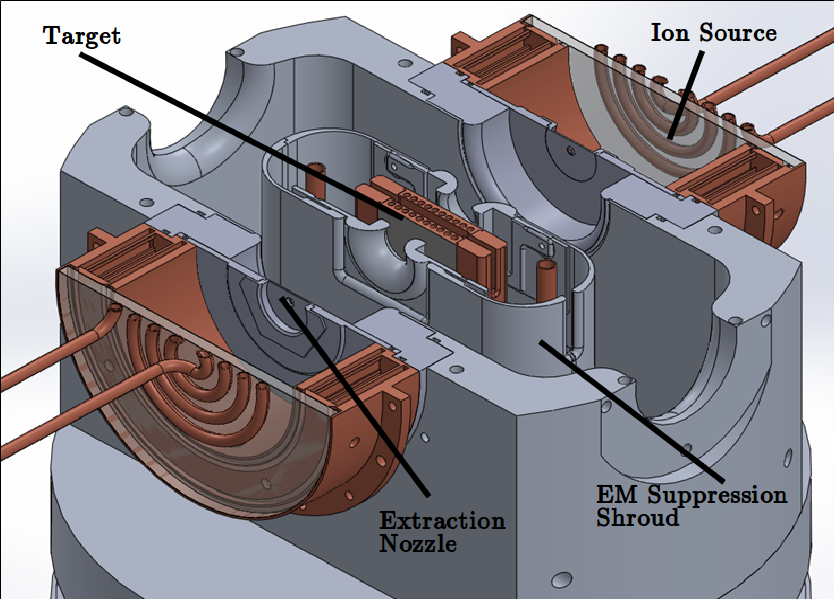
\includegraphics[width=\textwidth]{./figures/target2.png}
        \subfigimg[width=0.5\textwidth]{}{./figures/87mY.pdf}{50}
%         \caption{Decay curve for the $\beta^-$ decay of \ce{^{116}In}.}
        %         \refstepcounter{subfigure}
%          \label{fig:87mY}
%    }
%     \subfloat{
%         \centering
%         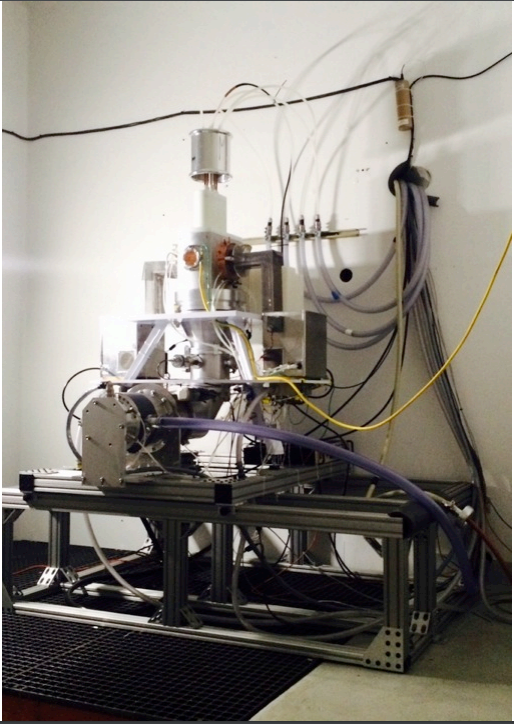
\includegraphics[width=\columnwidth]{./figures/Capture.PNG}
        \subfigimg[width=0.5\textwidth]{}{./figures/87Zr.pdf}{50}
%         \caption{ Decay curve for the $\beta^+$ decay of \ce{^{64}Cu}.}
%         \refstepcounter{subfigure}
%         \label{fig:87Zr}
   \hspace{-10pt}}%
    \\
    \subfloat{
        \centering
%         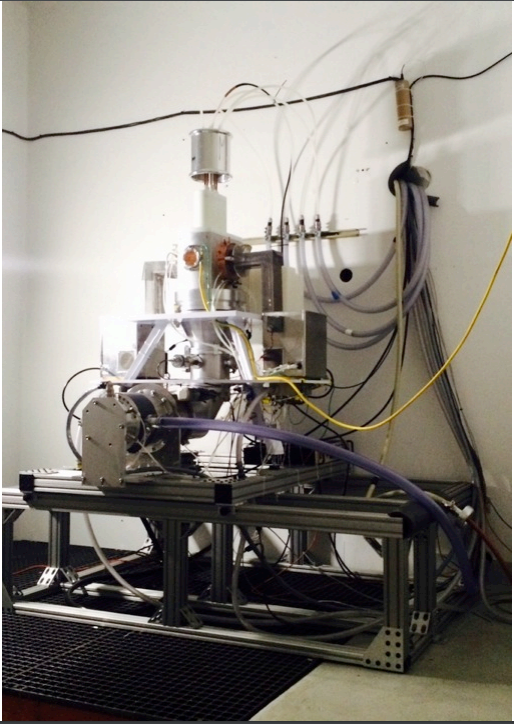
\includegraphics[width=\columnwidth]{./figures/Capture.PNG}
        \subfigimg[width=0.5\textwidth]{}{./figures/88Y.pdf}{50}
%         \caption{ Decay curve for the isomeric transition of \ce{^{115m}In}.}
%         \refstepcounter{subfigure}
%          \label{fig:88Y}%
%         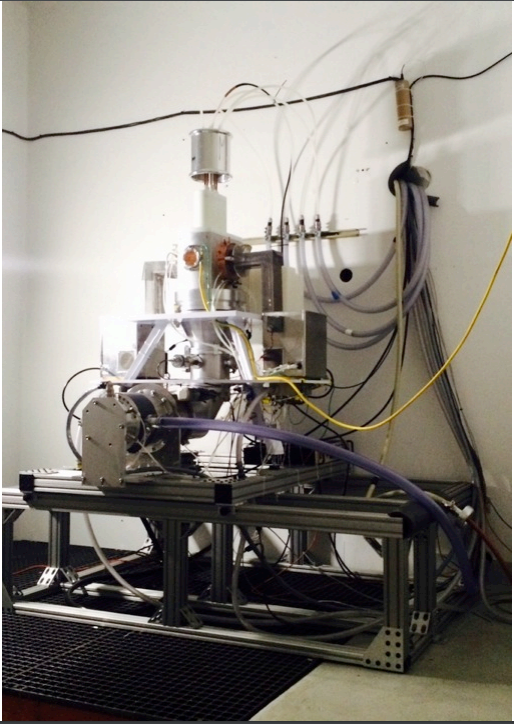
\includegraphics[width=\columnwidth]{./figures/Capture.PNG}
%         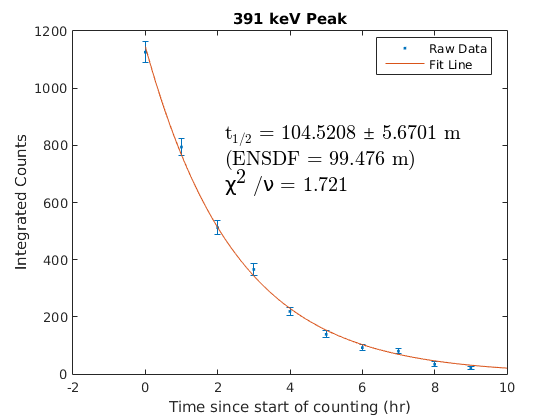
\includegraphics[scale=0.6]{./figures/391keV_curve2.png}
        \subfigimg[width=0.5\textwidth]{}{./figures/88Zr.pdf}{50}
%         \caption{ Decay curve for the isomeric transition of \ce{^{113m}In}.}
%         \refstepcounter{subfigure}
%          \label{fig:88Zr}
   \hspace{-10pt}}%
    \\
         \subfloat{
        \centering
%         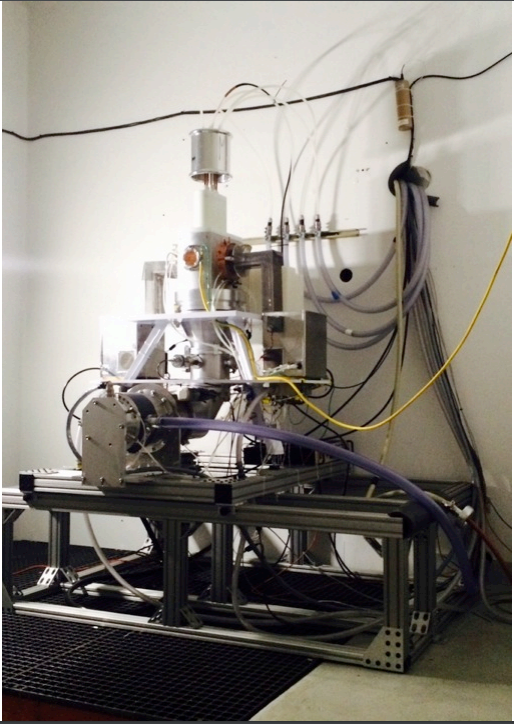
\includegraphics[width=\columnwidth]{./figures/Capture.PNG}
%         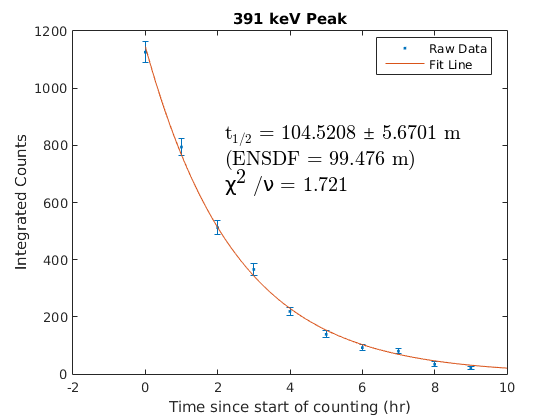
\includegraphics[scale=0.6]{./figures/391keV_curve2.png}
        \subfigimg[width=0.5\textwidth]{}{./figures/89Nb.pdf}{50}
%         \caption{ Decay curve for the isomeric transition of \ce{^{113m}In}.}
%         \refstepcounter{subfigure}
%          \label{fig:89Nb}
%    }%
%     \subfloat{
%         \centering
%         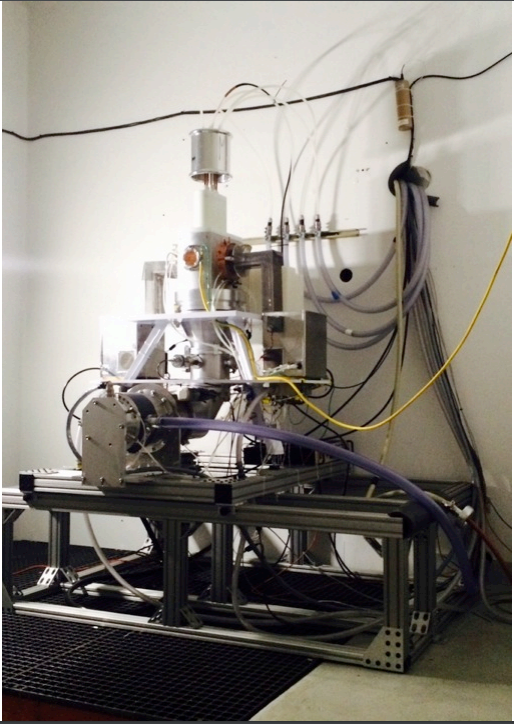
\includegraphics[width=\columnwidth]{./figures/Capture.PNG}
%         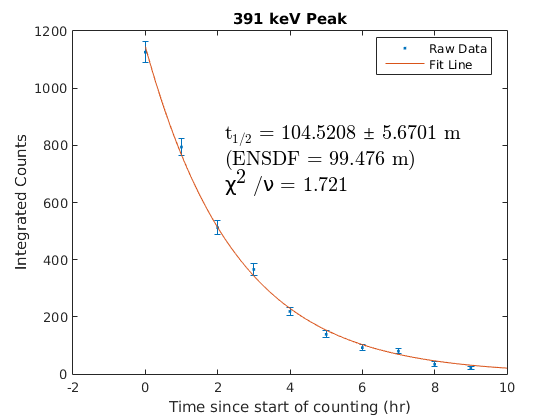
\includegraphics[scale=0.6]{./figures/391keV_curve2.png}
        \subfigimg[width=0.5\textwidth]{}{./figures/89gNb.pdf}{50}
%         \caption{ Decay curve for the isomeric transition of \ce{^{113m}In}.}
%         \refstepcounter{subfigure}
%          \label{fig:89gNb}
   \hspace{-10pt}}%
%     \caption{Decay curves used to verify photopeak transition assignment. (a) Decay curve for the isomeric transition of \ce{^{115m}In}, (b) decay curve for the isomeric transition of \ce{^{113m}In}, (c) decay curve for the $\beta^-$ decay of \ce{^{116}In}, and (d) decay curve for the $\beta^+$ decay of \ce{^{64}Cu}.}
     \phantomcaption{}\label{fig:xs_curves_p8}
\end{figure*}

\begin{figure*}
    \centering    
         \subfloat{
        \centering
% %         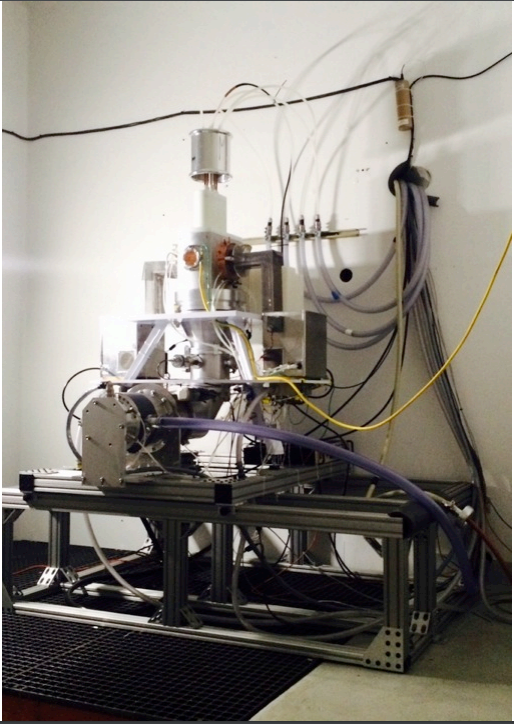
\includegraphics[width=\columnwidth]{./figures/Capture.PNG}
% %         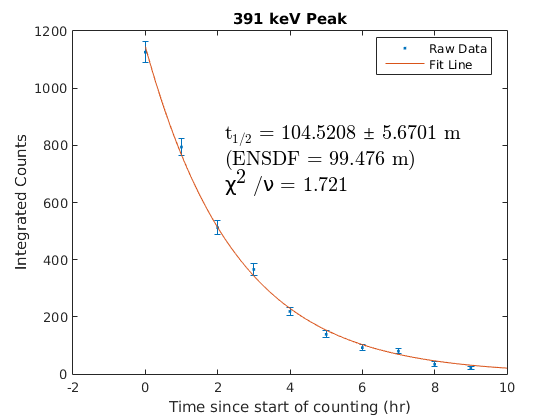
\includegraphics[scale=0.6]{./figures/391keV_curve2.png}
%         \subfigimg[width=0.5\textwidth]{}{./figures/89gNb.pdf}{50}
% %         \caption{ Decay curve for the isomeric transition of \ce{^{113m}In}.}
% %         \refstepcounter{subfigure}
%          \label{fig:89gNb}
% %    }%
%     \subfloat{
%         \centering
%         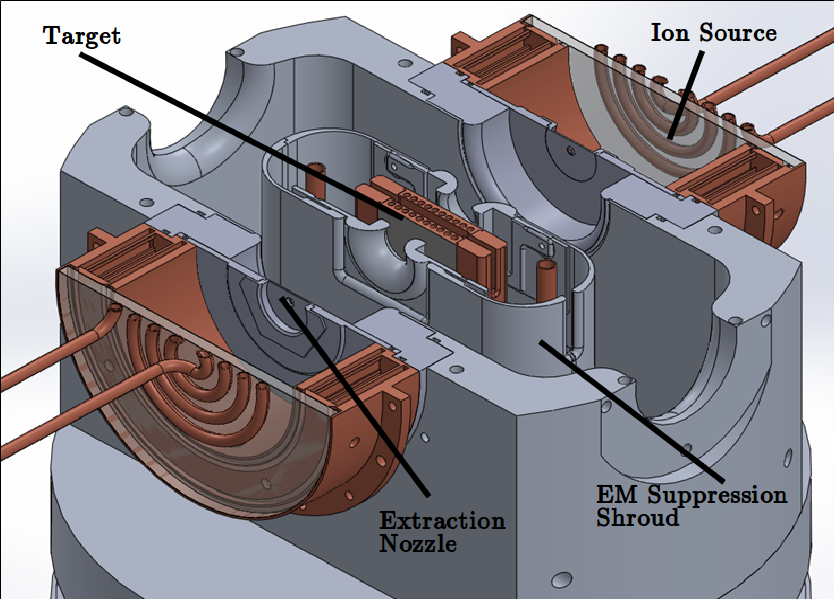
\includegraphics[width=\textwidth]{./figures/target2.png}
        \subfigimg[width=0.5\textwidth]{}{./figures/89mNb.pdf}{50}
%         \caption{Decay curve for the $\beta^-$ decay of \ce{^{116}In}.}
        %         \refstepcounter{subfigure}
%          \label{fig:89mNb}
%    }
%      \subfloat{
%         \centering
%         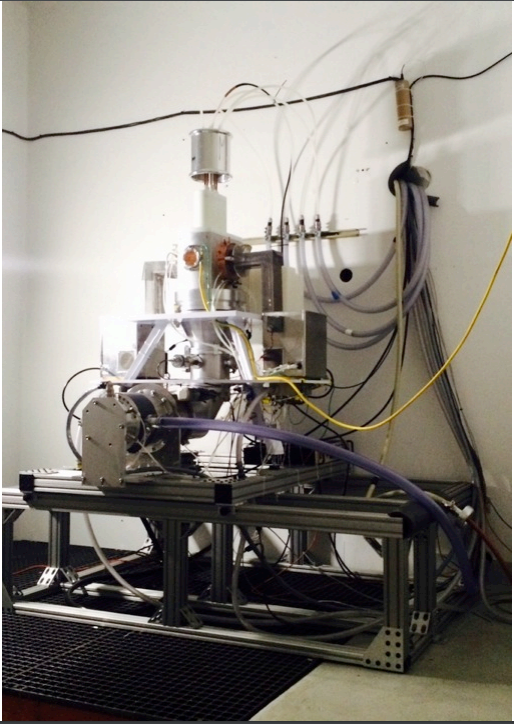
\includegraphics[width=\columnwidth]{./figures/Capture.PNG}
        \subfigimg[width=0.5\textwidth]{}{./figures/89Zr.pdf}{50}
%         \caption{ Decay curve for the $\beta^+$ decay of \ce{^{64}Cu}.}
%         \refstepcounter{subfigure} 
%         \label{fig:89Zr}
   \hspace{-10pt}}%
    \\
    \subfloat{
        \centering
%         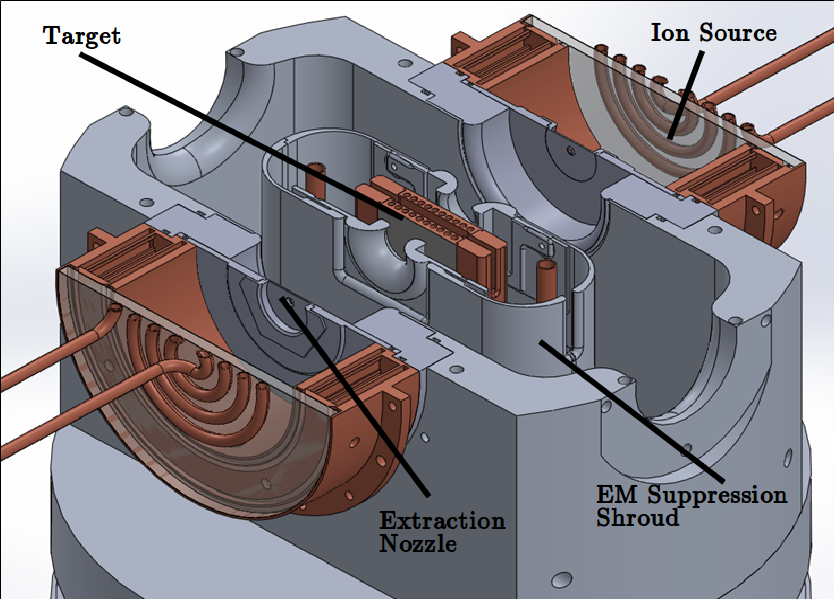
\includegraphics[width=\textwidth]{./figures/target2.png}
        \subfigimg[width=0.5\textwidth]{}{./figures/91mNb.pdf}{50}
%         \caption{Decay curve for the $\beta^-$ decay of \ce{^{116}In}.}
        %         \refstepcounter{subfigure}
%          \label{fig:91mNb}
%    }
%      \subfloat{
%         \centering
%         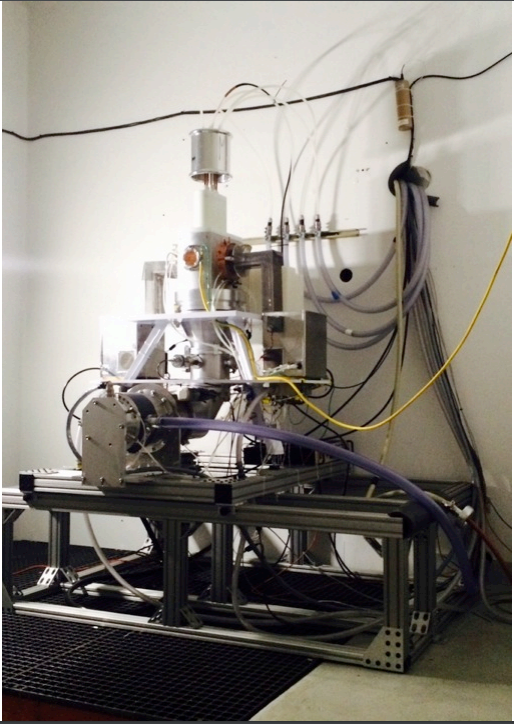
\includegraphics[width=\columnwidth]{./figures/Capture.PNG}
        \subfigimg[width=0.5\textwidth]{}{./figures/92mNb.pdf}{50}
%         \caption{ Decay curve for the $\beta^+$ decay of \ce{^{64}Cu}.}
%         \refstepcounter{subfigure} 
%         \label{fig:92mNb}
   \hspace{-10pt}}%
    \\
    \subfloat{
        \centering
%         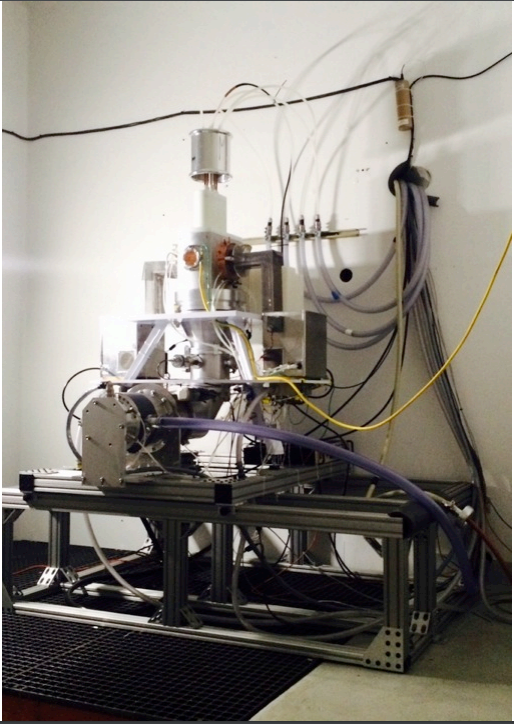
\includegraphics[width=\columnwidth]{./figures/Capture.PNG}
        \subfigimg[width=0.5\textwidth]{}{./figures/93mMo.pdf}{50}
%         \caption{ Decay curve for the isomeric transition of \ce{^{115m}In}.}
%         \refstepcounter{subfigure}
%          \label{fig:93mMo}
   }%
%     \caption{Decay curves used to verify photopeak transition assignment. (a) Decay curve for the isomeric transition of \ce{^{115m}In}, (b) decay curve for the isomeric transition of \ce{^{113m}In}, (c) decay curve for the $\beta^-$ decay of \ce{^{116}In}, and (d) decay curve for the $\beta^+$ decay of \ce{^{64}Cu}.}
     \phantomcaption{}\label{fig:xs_curves_p7}
\end{figure*}

% \begin{figure*}
%     \centering
%     \subfloat{
%         \centering
% %         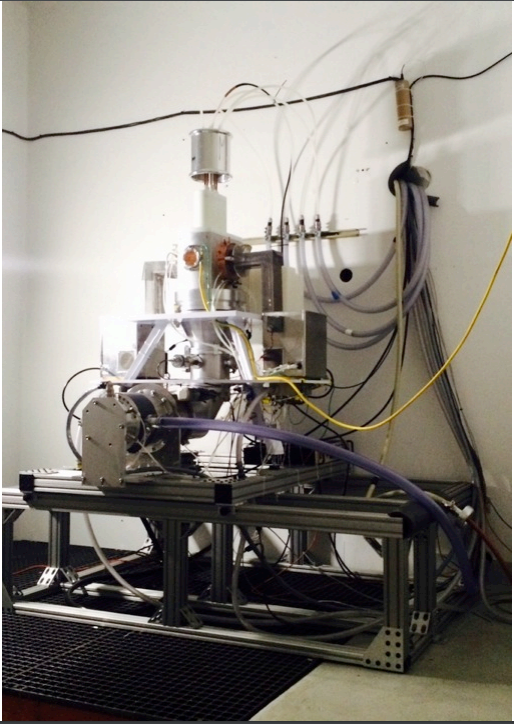
\includegraphics[width=\columnwidth]{./figures/Capture.PNG}
%         \subfigimg[width=0.5\textwidth]{}{./figures/93mMo.pdf}{50}
% %         \caption{ Decay curve for the isomeric transition of \ce{^{115m}In}.}
% %         \refstepcounter{subfigure}
%          \label{fig:93mMo}
%    }%
% %      \subfloat{
% %         \centering
% % %         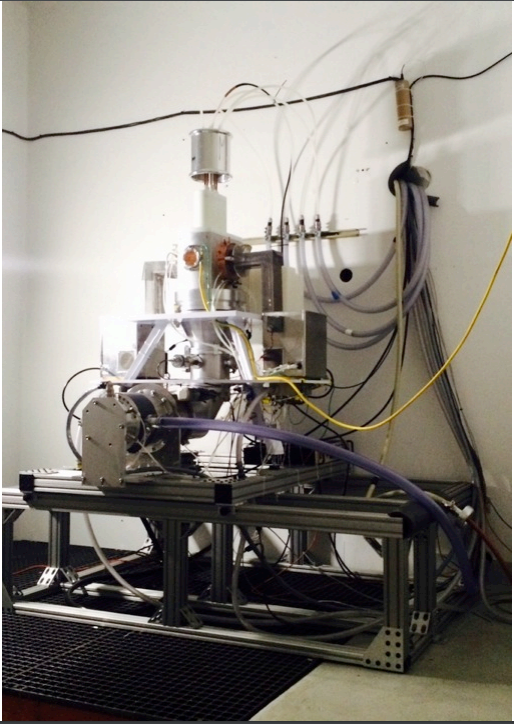
\includegraphics[width=\columnwidth]{./figures/Capture.PNG}
% % %         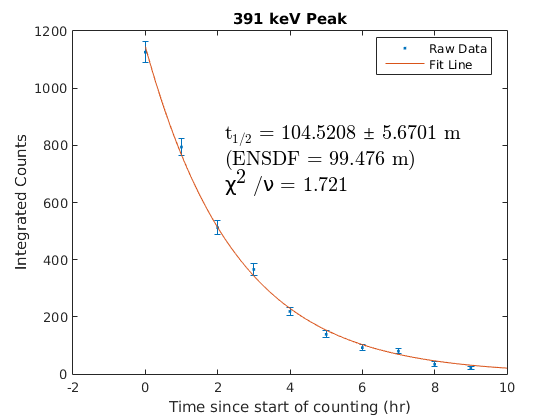
\includegraphics[scale=0.6]{./figures/391keV_curve2.png}
% %         \subfigimg[width=0.5\textwidth]{}{./figures/91mNb.pdf}{50}
% % %         \caption{ Decay curve for the isomeric transition of \ce{^{113m}In}.}
% % %         \refstepcounter{subfigure}
%          \label{fig:91mNb}
% %    }%
% %     \\
% %     \subfloat{
% %         \centering
% % %         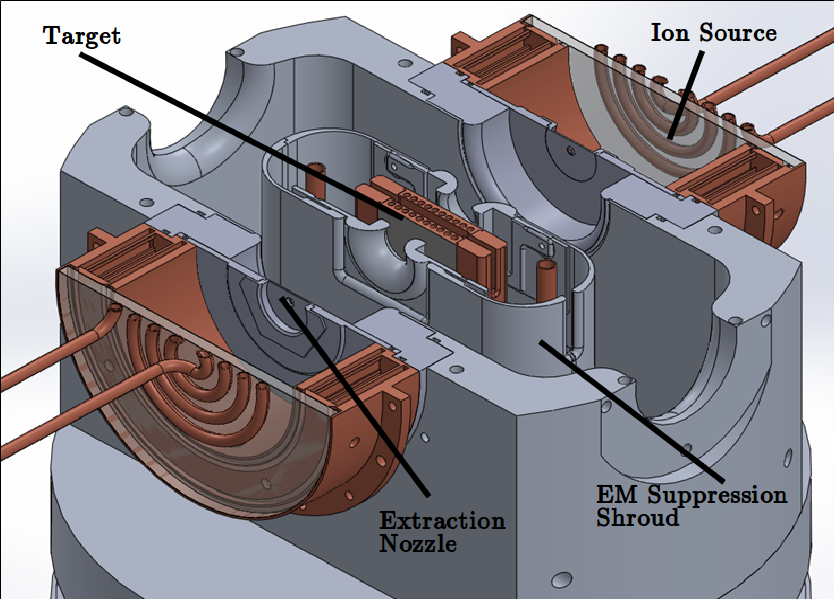
\includegraphics[width=\textwidth]{./figures/target2.png}
% %         \subfigimg[width=0.5\textwidth]{}{./figures/92mNb.pdf}{50}
% % %         \caption{Decay curve for the $\beta^-$ decay of \ce{^{116}In}.}
% %         %         \refstepcounter{subfigure}
%          \label{fig:92mNb}
% %    }
% %      \subfloat{
% %         \centering
% % %         \includegraphics[width=\columnwidth]{./figures/Capture.PNG}
% %         \subfigimg[width=0.5\textwidth]{}{./figures/93mMo.pdf}{50}
% % %         \caption{ Decay curve for the $\beta^+$ decay of \ce{^{64}Cu}.}
% %%         \refstepcounter{subfigure} \label{fig:93mMo}
% %    }%
% %     \caption{Decay curves used to verify photopeak transition assignment. (a) Decay curve for the isomeric transition of \ce{^{115m}In}, (b) decay curve for the isomeric transition of \ce{^{113m}In}, (c) decay curve for the $\beta^-$ decay of \ce{^{116}In}, and (d) decay curve for the $\beta^+$ decay of \ce{^{64}Cu}.}
%      \label{fig:xs_curves_p5}
% \end{figure*}




% 
% 
\section{Measured isomer-to-ground state branching ratios } \label{ibr_figures}

Plots of the isomer-to-ground state ratios measured in this work are presented here, in comparison with literature data and reaction modeling codes \cite{MICHEL1997153,Ditroi2008,Titarenko2011,Graves2016}.




% \begin{figure*}
%     \centering
%     \subfloat{
%         \centering
% %         \includegraphics[width=\columnwidth]{./figures/Capture.PNG}
%         \subfigimg[width=0.5\textwidth]{a)}{./figures/336keV_curve_new.pdf}{50}
% %         \caption{ Decay curve for the isomeric transition of \ce{^{115m}In}.}
% %          \refstepcounter{subfloat}
%          \label{fig:decay_curve_336}
% %          
%          \subfigimg[width=0.5\textwidth]{b)}{./figures/391keV_curve_new.pdf}{50}
% %         \caption{ Decay curve for the isomeric transition of \ce{^{113m}In}.}
% %          \refstepcounter{subfloat}
%          \label{fig:decay_curve_391}
%     }%
     

\begin{figure*}
    \centering
    \subfloat{
        \centering
%         \includegraphics[width=\columnwidth]{./figures/Capture.PNG}
        \subfigimg[width=0.5\textwidth]{}{./figures/52Mn_IBR.pdf}{50}
%         \caption{ Decay curve for the isomeric transition of \ce{^{115m}In}.}
%         \refstepcounter{subfigure}
%          \label{fig:52Mn_IBR}%
%         \includegraphics[width=\columnwidth]{./figures/Capture.PNG}
%         \includegraphics[scale=0.6]{./figures/391keV_curve2.png}
        \subfigimg[width=0.5\textwidth]{}{./figures/58Co_IBR.pdf}{50}
%         \caption{ Decay curve for the isomeric transition of \ce{^{113m}In}.}
%         \refstepcounter{subfigure}
%          \label{fig:58Co_IBR}
   \hspace{-10pt}}%
    \\
    \subfloat{
        \centering
%         \includegraphics[width=\textwidth]{./figures/target2.png}
        \subfigimg[width=0.5\textwidth]{}{./figures/85Y_IBR.pdf}{50}
%         \caption{Decay curve for the $\beta^-$ decay of \ce{^{116}In}.}
        %         \refstepcounter{subfigure}
%          \label{fig:85Y_IBR}
%    }
%      \subfloat{
%         \centering
%         \includegraphics[width=\columnwidth]{./figures/Capture.PNG}
        \subfigimg[width=0.5\textwidth]{}{./figures/87Y_IBR.pdf}{50}
%         \caption{ Decay curve for the $\beta^+$ decay of \ce{^{64}Cu}.}
%         \refstepcounter{subfigure} 
%         \label{fig:87Y_IBR}
   \hspace{-10pt}}%
    \\
    \subfloat{
        \centering
%         \includegraphics[width=\textwidth]{./figures/target2.png}
        \subfigimg[width=0.5\textwidth]{}{./figures/89Nb_IBR.pdf}{50}
%         \caption{Decay curve for the $\beta^-$ decay of \ce{^{116}In}.}
        %         \refstepcounter{subfigure}
%          \label{fig:89Nb_IBR}
   }
     \phantomcaption{}\label{fig:ibr_curves}
\end{figure*}
